%%%%%%%%%%%%%%%%%%%%%%%%%%%%%%%%%%%%%%%%%%%%%%%%%%%%%%%%%%%%%%%%%%%%%%%%%%%%%%%%
% Template for USENIX papers.
%
% History:
%
% - TEMPLATE for Usenix papers, specifically to meet requirements of
%   USENIX '05. originally a template for producing IEEE-format
%   articles using LaTeX. written by Matthew Ward, CS Department,
%   Worcester Polytechnic Institute. adapted by David Beazley for his
%   excellent SWIG paper in Proceedings, Tcl 96. turned into a
%   smartass generic template by De Clarke, with thanks to both the
%   above pioneers. Use at your own risk. Complaints to /dev/null.
%   Make it two column with no page numbering, default is 10 point.
%
% - Munged by Fred Douglis <douglis@research.att.com> 10/97 to
%   separate the .sty file from the LaTeX source template, so that
%   people can more easily include the .sty file into an existing
%   document. Also changed to more closely follow the style guidelines
%   as represented by the Word sample file.
%
% - Note that since 2010, USENIX does not require endnotes. If you
%   want foot of page notes, don't include the endnotes package in the
%   usepackage command, below.
% - This version uses the latex2e styles, not the very ancient 2.09
%   stuff.
%
% - Updated July 2018: Text block size changed from 6.5" to 7"
%
% - Updated Dec 2018 for ATC'19:
%
%   * Revised text to pass HotCRP's auto-formatting check, with
%     hotcrp.settings.submission_form.body_font_size=10pt, and
%     hotcrp.settings.submission_form.line_height=12pt
%
%   * Switched from \endnote-s to \footnote-s to match Usenix's policy.
%
%   * \section* => \begin{abstract} ... \end{abstract}
%
%   * Make template self-contained in terms of bibtex entires, to allow
%     this file to be compiled. (And changing refs style to 'plain'.)
%
%   * Make template self-contained in terms of figures, to
%     allow this file to be compiled. 
%
%   * Added packages for hyperref, embedding fonts, and improving
%     appearance.
%   
%   * Removed outdated text.
%
%%%%%%%%%%%%%%%%%%%%%%%%%%%%%%%%%%%%%%%%%%%%%%%%%%%%%%%%%%%%%%%%%%%%%%%%%%%%%%%%

%%% Minor updates for SOUPS 2019 by Michelle Mazurek

\documentclass[letterpaper,twocolumn,10pt]{article}
\usepackage{usenix2021_SOUPS}

% to be able to draw some self-contained figs
\usepackage{tikz}
\usepackage{amsmath}

% inlined bib file
\usepackage{filecontents}

%-------------------------------------------------------------------------------
\begin{filecontents}{\jobname.bib}
%-------------------------------------------------------------------------------
@inproceedings {197318,
author = {Shrirang Mare and Mary Baker and Jeremy Gummeson},
title = {A Study of Authentication in Daily Life},
booktitle = {Twelfth Symposium on Usable Privacy and Security (SOUPS 2016)},
year = {2016},
isbn = {978-1-931971-31-7},
address = {Denver, CO},
pages = {189--206},
url = {https://www.usenix.org/conference/soups2016/technical-sessions/presentation/mare},
publisher = {USENIX Association},
month = jun,
}
@article{lillegaard,
author = {Lillegaard, Inger and Løken, E and Andersen, Lene},
year = {2007},
month = {02},
pages = {61-8},
title = {Relative validation of a pre-coded food diary among children, under-reporting varies with reporting day and time of the day},
volume = {61},
journal = {European journal of clinical nutrition},
doi = {10.1038/sj.ejcn.1602487}
}
\end{filecontents}

%-------------------------------------------------------------------------------
\begin{document}
%-------------------------------------------------------------------------------

%don't want date printed
\date{}

% make title bold and 14 pt font (Latex default is non-bold, 16 pt)
\title{\Large \bf A Study of Authentication in Daily Life of University Students}

% if you leave this blank it will default to a possibly ugly attempt 
% to make the contents of the \author command below into a string
\def\plainauthor{Author name(s) for PDF metadata. Don't forget to anonymize for submission!}

%for single author (just remove % characters)
\author{
{\rm Rakshit Bhat}\\
University Paderborn
\and
{\rm Nidhi Nadig}\\
University Paderborn
% copy the following lines to add more authors
\and
{\rm Subramanya Padmaraja Setty}\\
University Paderborn
\and
{\rm Mayank Kapadi}\\
University Paderborn
\and
{\rm Pritom Touhid Hossain}\\
University Paderborn
\and
{\rm Showmik Md Jannatul Baki}\\
University Paderborn
} % end author

\maketitle
\thecopyright

%-------------------------------------------------------------------------------
\begin{abstract}
%-------------------------------------------------------------------------------
We are surveying 20 people to determine the usability of the daily authentication techniques on different authentication devices. We determine various target devices, including phones, PCs, websites, doors, Tablets, etc. with various authenticators like passwords, PINs, physical keys, Physical tokens, fingerprints, etc. Our research focuses on determining how stressful managing different authentication techniques are and improving these techniques to benefit the users and the companies.
\end{abstract}


%-------------------------------------------------------------------------------
\section{Introduction}
%-------------------------------------------------------------------------------
Many of us carry a lot of authentication devices with us in our daily life. These devices include a car key, house key, corporate badge, bike key, RSA token, bus pass, credit card, driver's license, ATM card \cite{197318}. We also remember the passwords and use fingerprints and faceiDs to unlock the devices. These are called authenticators, tools for authentications or confirming the user's identity. By proving that they are in control of an authenticator, a person authenticates to a computer system or application. Recent studies have found that it is burdensome, and there is no insight into current authentication habits and burdens. To fill out this gap, we replicate the study by Mare et al. \cite{197318} and focus only on university students for our survey. To carry out the survey, we have developed a tool in the form of a mobile application% 
\footnote{Github URL: https://github.com/rakshitongit/usap-survey} to log the participants' data. \\
\textbf{Types of authentications:} We summarised a few most common authentication techniques that users use daily. These include security questions, Passwords, Pins, SMS voice or email OTPs, Push notifications, Physical tokens, and Biometrics.

Today, it has become very stressful for users with so many different types of authentication techniques available.  Users have questions like whom to trust or which of these authentication types is more secure. There are some problems with these authentication techniques; if you enable 2-factor authentication and lose the device responsible for that, you will not be able to authenticate further. Witty et al. \cite{} concluded from their research that it takes around \$50 - \$150 to resolve issues and reset passwords. We investigate the following research questions to determine the usability of the authentication in daily life. 
\begin{enumerate}
    \item What are the university students' various types of authentication techniques?
    \item How much of a burden is it to authenticate in their daily life?
    \item How failure-prone are the different types of authentication? 
    \item Does the general public concur on the types of authentication they prefer or not?
\end{enumerate}

To tackle these queries, we conducted a wearable digital diary user survey of 20 people, which included university students, to better understand the user authentication burden. We chose university students because it became easy for them to explain the purpose of our research, and we quickly got some volunteers to participate in our study. First, we conducted a pre-interview session with the university students, explained our study, and encouraged them to participate in the survey. People who agreed to participate needed to sign a consent form%
\footnote{Link: shorturl.at/jrzP6} to prove that our survey was ethically correct to the participants. The university students then completed the survey by logging their authentication data for four days. After the survey, we conducted a post-logging interview to determine the study and get feedback from them. We did a qualitative analysis based on the post-logging sessions. 

%-------------------------------------------------------------------------------
\section{Related Work}
%-------------------------------------------------------------------------------

Footnotes should be places after punctuation characters, without any
spaces between said characters and footnotes, like so.%
\footnote{Github URL: https://github.com/rakshitongit/usap-survey} And some embedded literal code may
look as follows.

\begin{verbatim}
int main(int argc, char *argv[]) 
{
    return 0;
}
\end{verbatim}

Now we're going to cite somebody. Watch for the cite tag. Here it
comes. Arpachi-Dusseau and Arpachi-Dusseau co-authored an excellent OS
book, which is also really funny~\cite{arpachiDusseau18:osbook}, and
Waldspurger got into the SIGOPS hall-of-fame due to his seminal paper
about resource management in the ESX hypervisor~\cite{waldspurger02}.

The tilde character (\~{}) in the tex source means a non-breaking
space. This way, your reference will always be attached to the word
that preceded it, instead of going to the next line.

And the 'cite' package sorts your citations by their numerical order
of the corresponding references at the end of the paper, ridding you
from the need to notice that, e.g, ``Waldspurger'' appears after
``Arpachi-Dusseau'' when sorting references
alphabetically~\cite{waldspurger02,arpachiDusseau18:osbook}. 

It'd be nice and thoughtful of you to include a suitable link in each
and every bibtex entry that you use in your submission, to allow
reviewers (and other readers) to easily get to the cited work, as is
done in all entries found in the References section of this document.

Now we're going take a look at Section~\ref{sec:figs}, but not before
observing that refs to sections and citations and such are colored and
clickable in the PDF because of the packages we've included.

%-------------------------------------------------------------------------------
\section{Methodology}
\label{sec:method}
%-------------------------------------------------------------------------------


%---------------------------

%% %---------------------------

In this section, we will discuss the Authentication event (what kind of data will the participants log) and the Digital diary (how will the participant log the data)

\subsection{Authentication event}
The participants must log the authentication data each time they do an authentication event. To define the term authentication event, we did some research on the previous researchers \cite{197318} and replicated it. Mare et al. \cite{197318} have defined the authentication event as where the participants must verify that they are the appropriate people to access typical resources or services through something they are or something they have. Examples include unlocking a mobile or tablet device, a house door, login to a website or banking transactions, etc. Although, we do not consider lock or re-lock as an authentication event. We now define an authentication target as a device, a resource or service through which the user can request access, and an authenticator as proof that the user needs to provide to gain access. Consider an example of users unlocking their mobile phones with their fingerprints. Here mobile phones are authentication target devices, and fingerprint/biometrics are authenticators. Similarly, opening a house door with a key, the door is the authentication target device, and the house key is the authenticator. Some more examples of authenticators and authentication target. \\ \\
\noindent
\textbf{Authentication Targets:} Computers (Laptop, desktops), Mobile Phone, Tablet (also e-readers), Website (also online websites or any software), Door, Car, ATM, Bicycle (also motorcycle), Phone payment, Card payment, Bank check, Locker (also locked drawers), and Other.
\\ \\
\noindent
\textbf{Authenticators:} Password (locker combinations, etc.), PINS, Biometrics (Fingerprint, Face biometrics, Voice biometrics), Card (ID cards, credit cards, badges), Physical tokens (Certificate (PKI)), Mouse click (where the participant has to click to authenticate, e.g., to request autofill with a password manager), Lock key (physical key), Signature, 2-Factor authenticators, and Other%
\footnote{These are general authenticators and authentication target devices which are being used by many users.}.

\begin{enumerate}
    \item \textbf{Security Questions:} These are some personal questions which are being asked by the Software to identify the users and verify them.
    \item \textbf{Passwords:} Softwares use classical passwords, secret words, or a group of words to verify the user. 
    \item \textbf{Pins:} These are usually numbers used in mobiles or laptops as an alternative to the passwords for quick login. 
    \item \textbf{OTPs:} OTP or One-time password means Software will send a password on your devices like mobiles or laptops via SMS or emails.
    \item \textbf{Push notifications:} This is one of the latest forms of the authentication technique in which the users need first to configure their mobile devices with the Software. Later while authenticating the user, the Software will send a push notification to the registered mobile device wherein the user can confirm and log in. 
    \item \textbf{Physical tokens:} These are physical keys encrypted using cryptographic algorithms and randomly generated each time the user wants to authenticate.
    \item \textbf{Biometrics:} These include fingerprints, voice recognition, face IDs etc., specially designed to recognise the user uniquely.
\end{enumerate}

In the survey, we are also interested in knowing the authentication location and the time the authentication takes place. We are also interested in the number of attempts before successful authentication and the convenience of the authentication events. Therefore, our authentication event is a tuple consisting of \{\textit{authentication-location, authentication-time, authentication target, authenticator, authentication-success, authentication-convenience}\}
\subsection{Digital Diary}
\begin{figure}
\begin{center}
  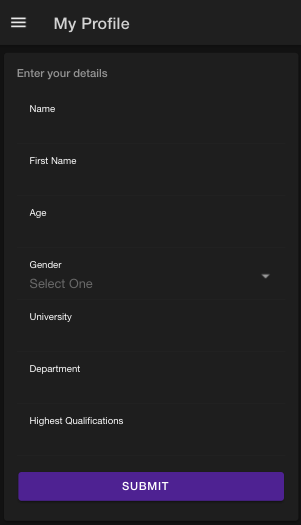
\includegraphics[scale=0.5]{images/profile.png}
\end{center}
\caption{\label{fig:app-profile} Mobile application - User Profile}
\end{figure}
\begin{figure}
\begin{center}
  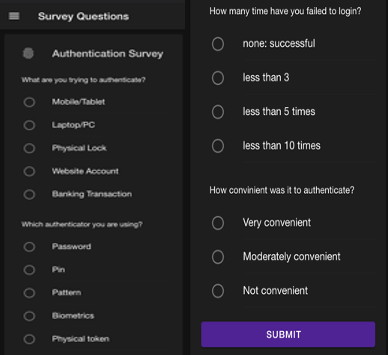
\includegraphics[scale=0.5]{images/main-survey-1.png}
\end{center}
\caption{\label{fig:app-main-survey} Mobile application - Main Survey}
\end{figure}
Lillegaard et al. \cite{lillegaard} suggested that digital dairies are a practical way to immediately and easily log events. Digital diaries are especially useful for events like authentication, which happen repeatedly and pulling out a paper notebook and pen or using a physical journal is difficult. Therefore, we developed a mobile application%
\footnote{Github URL: https://github.com/rakshitongit/usap-survey} that is easy to use and download for android users. For the other users, we deployed the webview%
\footnote{URL: https://n5lis62ifu.appflowapp.com/} of the mobile app. As shown in Figure \ref{fig:app-profile}, the participants must first fill up some of their personal data. As soon as they fill in this information, the participants are permitted to start with the survey. The survey page contains various types of questions (see Figure \ref{fig:app-main-survey}). The participant cannot submit unless all the questions are answered. The mobile application automatically collects the location (latitude and longitude) and the timestamp at which the participant has logged the data. In the neighbouring tab (see Figure \ref{fig:app-daily-survey}), the participant can find the daily questions, which the participant needs to fill in for the feedback and the qualitative data analysis. For an authentication event, we want to collect the authentication target, the authenticator, success or failure, number of attempts required (in case of success), location, and time. The app automatically collects GPS location and time, but participants must log the other four details. Event logging should be quick and straightforward to minimise disruption to the participants' ongoing tasks. If not, they will probably put off logging in and could forget to do so later. So, we came up with a mobile app which has only four questions and is easy to use. Some participants liked the interface of the app, while some suggested some improvements to the mobile app. We did several iterations of the mobile app development and finally came up with the interface seen in Figure \ref{fig:app-daily-survey} \& \ref{fig:app-main-survey}. The first question is to determine the authentication target, i.e. what is the participant trying to authenticate. We had five options: \texttt{Mobile/Tablet}, \texttt{Laptop/PC}, \texttt{Physical lock}, \texttt{Web application}, and \texttt{Banking transaction}. The second question determined the authenticator used by the participants, i.e. how the participants were authenticating the target device. We had six options: \texttt{Password}, \texttt{Pin}, \texttt{Patterns}, \texttt{Biometrics} (this included \textit{Voice}, \textit{Gait}, \textit{Heartbeat}, \textit{Eye-tracking}, \textit{Brain Waves}, \textit{Fingerprint}, and \textit{Iris scan}), \texttt{Physical Tokens}, and any \texttt{other} form of an authenticator. The third question determined the \textit{success/failure} and the number of times needed to authenticate. The options included: \texttt{None} (which meant success), \texttt{Less than 3}, \texttt{Less than 5}, and \texttt{Less than 10}.
The final question determined the convenience of the authentication. The options included: \texttt{Very convenient}, \texttt{Moderately convenient} and \texttt{Not convenient}. With this question, we would like to assess the usability of the authentication technique. In the pilot study, where we selected two people to log the data and get their feedback, they told us that they use many electronic devices and have various biometric techniques to log in to their devices. The options were a lot, so we decided to generalise them to an option "Biometrics''. Similarly, we explained to the users the other options in the pre-logging sessions. E.g. three people did not know what physical tokens are, so we gave them an overview. 
\begin{figure}
\begin{center}
  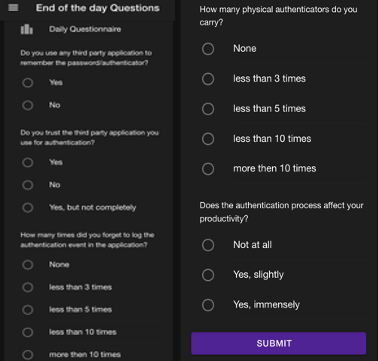
\includegraphics[scale=0.5]{images/eod-survey.png}
\end{center}
\caption{\label{fig:app-daily-survey} Mobile application - Daily Survey}
\end{figure}
\subsection{Study procedure}
We did a person one-day pilot study to test the smartphone mobile application. We got specific User Interface (UI) related feedback from them, and then we fixed a few issues. We then executed our survey with an entire group of people.
\subsubsection{Recruitment and enrollment}
We recruited participants through word-of-mouth which included our friends, and their friends agreed to join this survey. We initially asked the participants if they were willing to do the study. We provided informed consent to all the participants. If they agreed to the approval, we invited them for a talk. We asked them to sign an ethical consent form affiliated with the University of Paderborn%
\footnote{Link: shorturl.at/jrzP6}. We explained to the participants what information we were going to collect. We told them we would collect their location and the timestamp apart from anything else visible on the mobile application. We also informed them that they could withdraw from the study at any time for any or no reason. We also warned participants about safe logging: "Please only log events on the phone when it is safe to do so. Please do not use the devices while driving, biking, crossing streets, operating heavy machinery, or anything else that would be risky!" 
We installed the smartphone app on participants' Android smartphones. If a participant did not have an Android smartphone, we created a web application which could run on a browser. The only disadvantage of the web application was it only was available for a week. The ethics committee approved our study at the University of Paderborn.
\subsubsection{Pre-logging interview}
We conducted a semi-structured one-to-one interview with the participants. Some of the interviews were in-person, while some had to be online. We used University Paderborn's Zoom%
\footnote{https://uni-paderborn-de.zoom.us/} and BigBlueButton%
\footnote{https://open-bbb.uni-paderborn.de/} accounts. It was a pre-study activity to learn about the participants' daily authentication activities, devices and resources they use, and authenticators they carry with them. We used a set of questions to guide these semi-structured interviews, which is available in the Appendix. We explained how to use our mobile applications and answered their questions and concerns. Some participants were concerned about sharing their data with a third party, but we mentioned that this would not be the case. 
\subsubsection{Post-logging interview}
We also conducted a one-to-one post-logging interview with the participants after two days of self-logging. We asked them about some authentication activities they did not understand, some ambiguity or concerns about authentication, any logged entry we did not understand, and authentication failure events. Most people remembered why their authentication activity failed, but some forgot why it failed. We also asked them about the UI of the mobile application, their choice of the worst and best authenticator, and the changes they want in the area of authentication.  We have the questions asked to the participants in the post-logging interview sessions in the Appendix section. 
\section{LIMITATIONS}
\subsection{Methodology successes and failures}
\section{FINDINGS}
\subsection{Results}
Explain about Qualitative and/or quantitative analysis
\subsection{Authentication burden}
%-----------------------------------
Explain how authentication has become a burden to the people

%-------------------------------------------------------------------------------
\section{Conclusion}
\section*{Acknowledgments}
%-------------------------------------------------------------------------------
Acknowledging the participants for their time...

%-------------------------------------------------------------------------------
\bibliographystyle{plain}
\bibliography{\jobname}

%%%%%%%%%%%%%%%%%%%%%%%%%%%%%%%%%%%%%%%%%%%%%%%%%%%%%%%%%%%%%%%%%%%%%%%%%%%%%%%%
\end{document}
%%%%%%%%%%%%%%%%%%%%%%%%%%%%%%%%%%%%%%%%%%%%%%%%%%%%%%%%%%%%%%%%%%%%%%%%%%%%%%%%

%%  LocalWords:  endnotes includegraphics fread ptr nobj noindent
%%  LocalWords:  pdflatex acks
